\chapter{Introduction}
\chapter{Introduction}

In this chapter we present the main features of a turbulent flow, providing an historical background of the direct numerical simulation field applied at the channel flow.

\section{Turbulent flows}
Every smoker can observe the nature of turbulence one inch away from their nose.
However a proper definition of turbulence is not yet given, due to the complexity of turbulence behaviour. \par
To use Prandtl words, who began an important lecture as follows: \\~\\
\emph{``What I am about to say on the phenomena of turbulent flows is still far from conclusive. It concerns, rather, the first steps in a new path which I hope will be followed by many others. The researches on the problem of turbulence which have been carried on at G\"{o}ttingen for about five years have unfortunately left the hope of thorough understanding of turbulent flow very small. The photographs and kinetographic pictures have shown us only how hopelessly complicated this flow is.''} \\~\\

Nowadays we can entrust to computational units that allows us to be no longer \emph{``hopeless''} as Prandtl was, although we are still far from having a solution, or at least a unique definition, of what the turbulence is. 
At the present time we define the turbulence as a flow regime, characterized by high Reynolds numbers and the presence of high level of diffusivity and irregularity, dissipation and three dimensional chaotic fluctuations in space and time\cite{turbulence:def}.


\section{General concepts}
An elderly definition of turbulence was provided by Hinze~\cite{Hinze}, in 1959, and say:\\~\\
\emph{``Turbulent fluid motion is an irregular condition of flow in which the various quantities show a random variation with time and space coordinates, so that statistically distinct average values can be discerned''}.\\~\\
The concept of \emph{average} is the keyword that humanity has used to start digging into the turbulence mysteries.
This kind of process, with its high sensitivity to the boundaries and initial conditions, can be defined as chaotic, so it can not be treated with a deterministic approach, therefore such randomness can be handled only by using a statistical approach.
In fact turbulence recovers its deterministic side inside statistical analysis: the detailed properties of the signal show a non predictable behaviour, but its statistical properties are consistent~\cite{Frisch}.
At statistical level, turbulent phenomena become reproducible and subject to systematic study, providing a basis for theoretical description. Therefore, the three-dimensional time-dependent Navier-Stokes equations can be solved and then the solution is averaged in order to obtain the statistics~\cite{Durbin}. 
\par
Note, however, that irregular motion and chaotic advection do not guarantee turbulence. Small point vortices can advect themselves in a chaotic manner or particles can follow complex trajectories, yet this is not turbulence. The definition, in fact, requires diffusivity. If the flow pattern looks random but does not exhibit high mix of momentum, mass and heat, it is surely not turbulent. Diffusivity is the single most important feature of turbulence, as highlighted by the experiment of Osborne Reynolds~\cite{Reynolds}, in 1883.
\par
In its famous work Reynolds has defined a ratio among inertia forces and viscous forces:
\begin{equation}
Re = \frac{ul}{\nu}
\end{equation}
\begin{figure}
\begin{center}
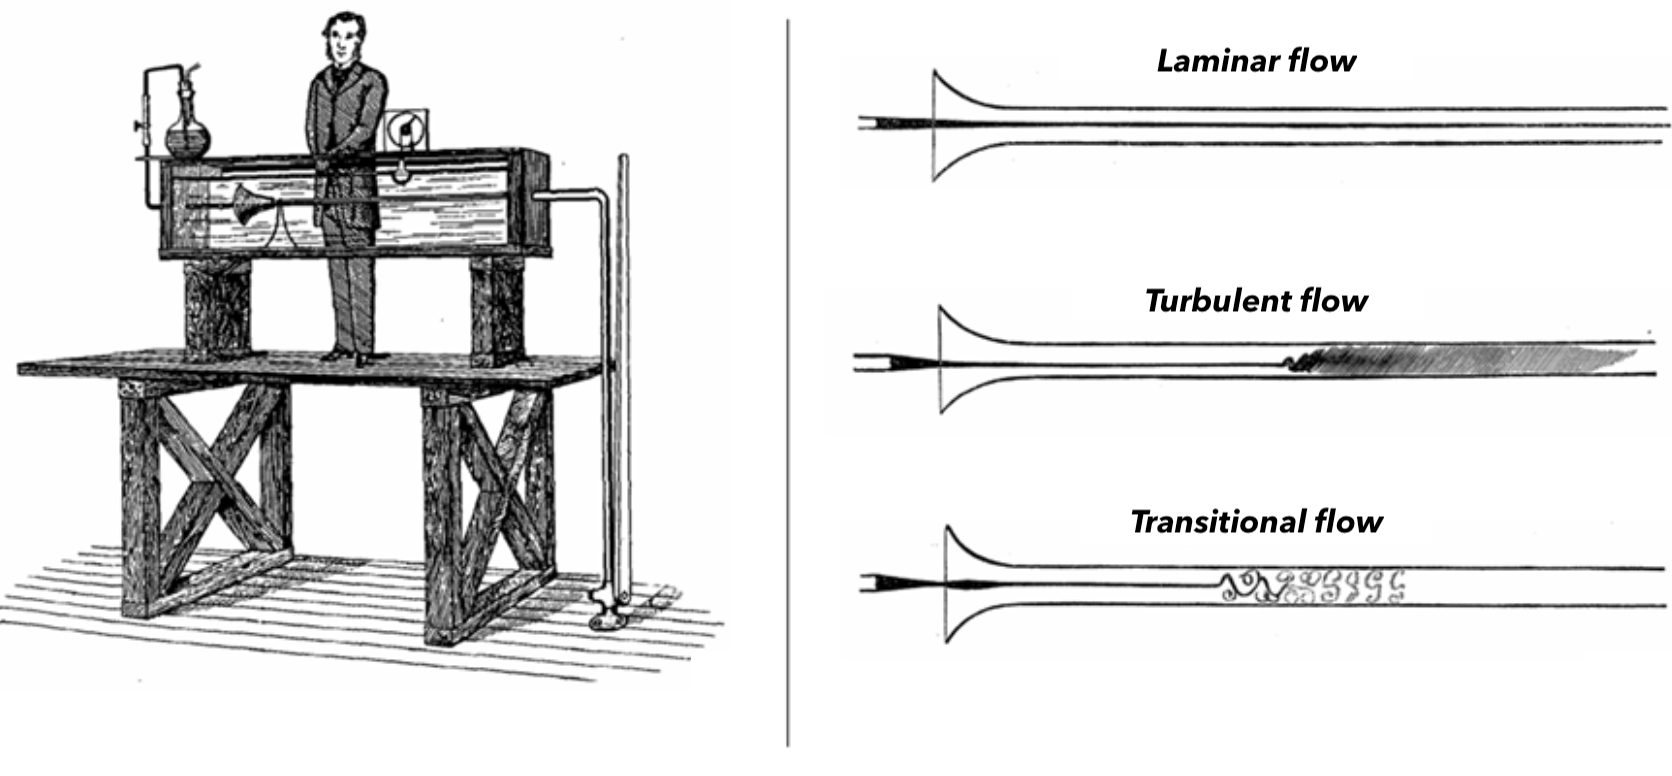
\includegraphics[width=1\textwidth]{grafici/reynolds_exp}
\caption{Sketch of the Reynolds experiment (\emph{left}) and flow patterns (\emph{right})}
\label{Reynolds:exp}
\end{center}
\end{figure}

with $u$ that is the characteristic velocity of the fluid, $l$ is the reference length of the scale and $\nu$ is the kinematic viscosity; able to predict the presence, or not, of the turbulence. He saw that when the inertia forces are huge the flow become unstable and the ink of its experiment started mixing with the surrounding water, as shown in the sketch of figure~\ref{Reynolds:exp}.
\par
This first work has correlated the presence of different states of the flow, laminar, transitional and turbulent, and their relationship with the couple viscous term-nonlinear inertia term.
Further observations revealed the presence of three-dimensional eddies. Although we are still unable to determine their shapes, we have understood that they play a key role in the turbulence sustenance. Under the assumptions of incompressible flow, not subjected to external forces of volume or surface, the vorticity equation states
\begin{equation}
\frac{D \boldsymbol{\omega}}{D t} = (\boldsymbol{\omega} \cdot \boldsymbol{\nabla})\boldsymbol{u} + \nu \boldsymbol{\nabla}^{2} \boldsymbol{u}.
\end{equation}
The central term of the equation, $ (\boldsymbol{\omega} \cdot \boldsymbol{\nabla})\boldsymbol{u}$, is known as vortex-stretching term. 
The vortex stretching is at the core of the description of the turbulent energy cascade, from the large scales to the smallest scale, determined, as we will see, by the turbulence itself.
For incompressible flow, due to volume conservation of fluid elements, the lengthening implies thinning of the fluid elements in the directions perpendicular to the stretching direction. This reduces the length scale of the associated vorticity. Finally, at the smallest scales the turbulence kinetic energy is dissipated into heat through the action of molecular viscosity~\cite{Lumley}.



\section{The history of the direct numerical simulation}
The direct numerical simulation (DNS) of the Navier-Stokes equations is a mathematical tool used to analyze turbulent flows since it allows to have an inner viewpoint in the transition and turbulence phenomena processes. It is part of the so called Computation Fluid Dynamics, or CFD, research field. 
Given the high computational cost of these simulations, DNS is not used to reproduce real-life flows, but as a research tool for flows with simple boundaries\cite{dns:tool}. \par
Despite of such kind of simulations, due to their limits, could seem useless, they assume relevant importance in the study of the turbulence, who, dominating the small scales, affect the behavior of the large scales, determining the raise of phenomenas such as flow separations, drag increases or losses of lift.
These simulations rely on high accuracy computational methods and they do not employ turbulence models, hence they require an ever-increasing computational power, as we move towards engineering relevant Reynolds numbers. 
However we can identify an ultimate threshold for direct numerical simulation of the wall bounded flows, which, thanks to its scale separation,  give the possibility to model the turbulence phenomena once for all. In~\cite{Jimenez2003} professor Jiménez set such threshold around $Re_{\tau}=10000$\\~\par




The DNS history is recent, with the first milestone work carried out by Kim, Moin and Moser~\cite{kim_moin_moser} in the 1987, using a $192\times 129 \times160$ grid of points distributed in a channel flow domain, in which they studied the homogenous isotropic turbulence using spectral modes. Follow this seminal work other authors proposed their simulations.
Accurate DNS calculations of the turbulent channel flow, using spectral methods, have been carried out by Lyons \emph{et al.}~\cite{Lyons}, Antonia \emph{et al.}~\cite{antonia_teitel_kim_browne_1992}, Kasagi \emph{et al.}~\cite{Kasagi}, Rutledge and Sleicher~\cite{Rutledge} in the first nineties. In the 1999 Moser \emph{et al.}~\cite{KMMans} proposed their $Re_{\tau}=590$ simulation, while to see the first channel flow simulation using finite differences we have to wait Abe \emph{et al.}~\cite{Abe} in 2001.\par
Other works, from the first years of the twenty-first century, are for example Iwamoto \emph{et al.}~\cite{Iwamoto} ones, Del Alamo and Jiménez~\cite{delalamo} and, the first simulation with $Re_{\tau}$ over a thousand, Del Alamo \emph{et al.}~\cite{delalamo2} work, in 2004. \par
Between 2004 and 2007 were presented different works, alternating the finite differences techniques with the more established spectral methods approach.
Tanahashi \emph{et al.}~\cite{Tanahashi}, Iwamoto \emph{et al.}~\cite{Iwamoto2}, Hoyas and Jiménez~\cite{Hoyas}, Hu \emph{et al.}~\cite{Hu}are some examples. \par
More recent simulation have been carried out by Lozano-Duràn \emph{et al.}~\cite{Lozano}, Lozano-Duràn and Jiménez~\cite{Lozano2}, Vreman and Kuerten~\cite{Vreman}, Bernardini \emph{et al.}~\cite{Bernardini} and the actually biggest simulation ever, with $Re_{\tau}=5200$, by Lee and Moser~\cite{Lee}. \par



The grows in $Re_{\tau}$ number is correlated with the grown in supercomputing performances on those years, as could be understood by looking at figures~\ref{top500} and~\ref{dns:trend}. However the $Re_{\tau}$ growth is not proportional with the computational power, as pointed out in~\cite{Jimenez2003}. In the same document is reported that a theoretical 500 Pflops supercomputer could carry out the $Re_{\tau}=10000$ simulation in a reasonable time. Unfortunately, starting from 2013, the rate of growth of the supercomputers speed has halved with respect to the past decade, and this made the forecast embedded in such document, false. With the current rate of growth it is more likely that we could carry out such simulation within the next three years. \\~\par



\begin{figure}
\begin{center}
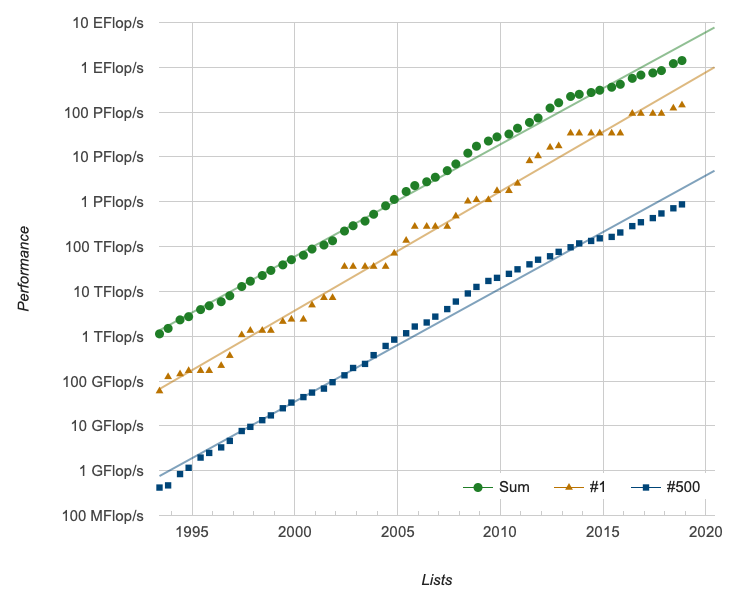
\includegraphics[width=0.8\textwidth]{grafici/top500hist}
\caption{Supercomputers grown trend, courtesy of TOP500.org}
\label{top500}
\end{center}
\end{figure}
\begin{figure}
\begin{center}
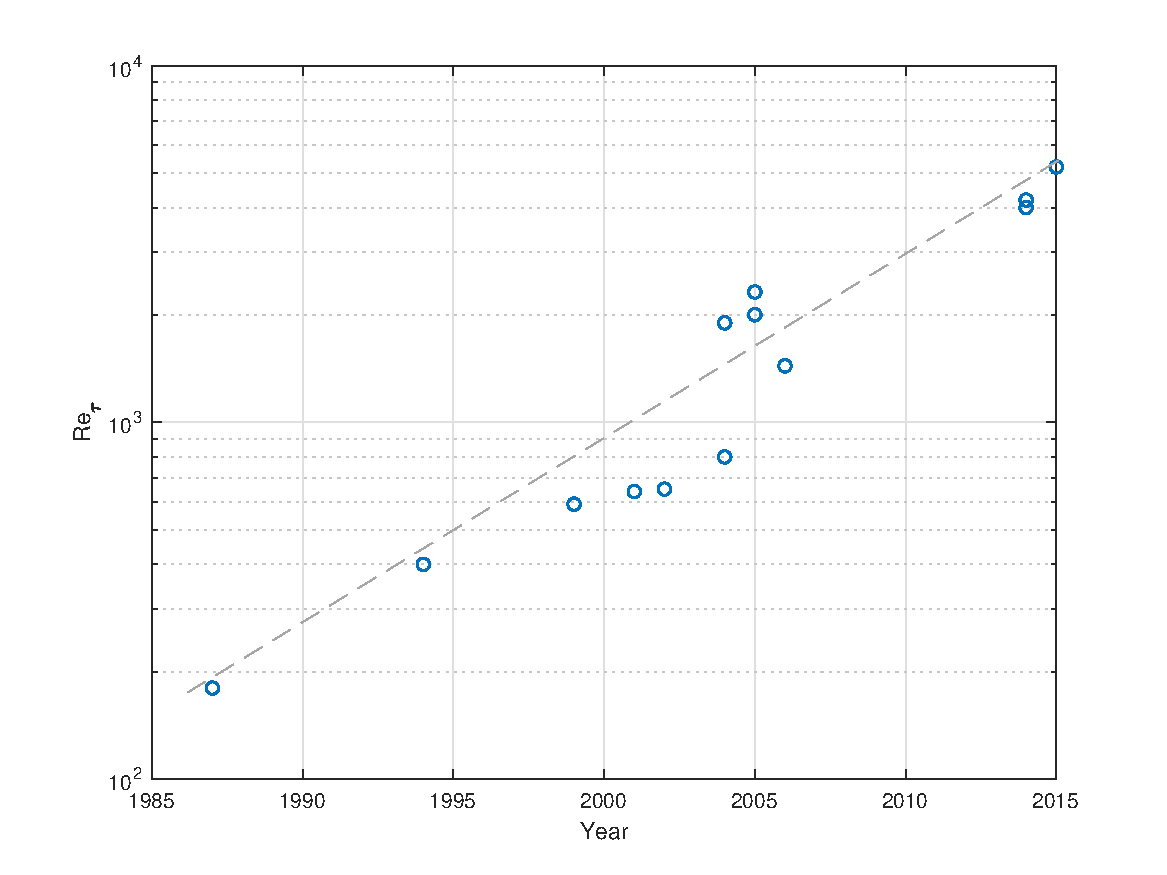
\includegraphics[width=0.8\textwidth]{grafici/dns_trend}
\caption{$Re_{\tau}$ grown trend}
\label{dns:trend}
\end{center}
\end{figure}



In this thesis our goal was to provide an highly parallelized DNS solver, based on pseudo-spectral approach, able to carry out simulation on a wide number of processors in the most efficient way possible. \par
We were particularly interested in the possibility to generate flow statistics at very high $Re_{\tau}$ values, in reasonable time, maintaining code efficiency above the 40\%. \\~\par

In this chapter we will provide a briefly description of the phenomena, then we will recall the main statistical quantities used to characterize turbulent flows. In the second chapter we will describe the geometry of the domain along with the governing equations for the problem presented, the structure of the code, discretization, domain decomposition and I/O.
The third chapter will deal with code benchmarks while the fourth will show the results of our simulations and the code validation against the well established $Re_{\tau}=180$ database of Kim, Moin and Moser. Finally we will draw a line of possible future works.






  




  



\section{Problem Definition}
\pagestyle{headings}

Before moving to what has been done in this thesis I wish to briefly discuss the setup of our channel flow and the equations used to solve the problem.

\begin{figure}[h]
\centering
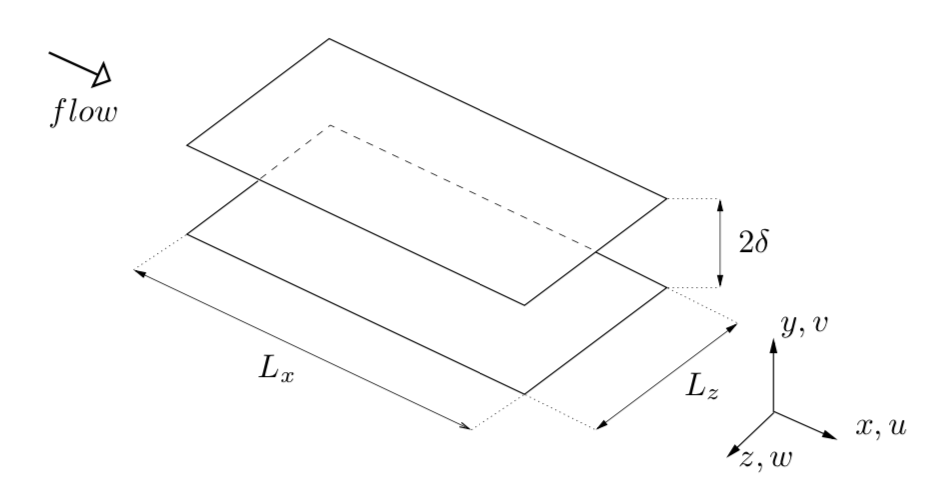
\includegraphics[width=0.8\textwidth]{grafici/sketch_dominio}
\caption{Domain of interest}
\label{sketch_dominio}
\end{figure}

We have the domain sketched in figure~\ref{sketch_dominio} where the $x$ and $z$ coordinates denote the streamwise and spanwise directions of the flow, while the $y$ coordinate is the wall normal ones.
Along these three dimension we have $u,v$ and $w$ components of velocity.

The flow is assumed to be periodic in the streamwise and spanwise directions. The lower wall is at position $y_l$ and the upper wall at position $y_u$. The reference length $\delta$ is taken to be one half of the channel height.
Once an appropriate reference velocity is chosen, we can define the Reynolds number as:
\[
Re = \frac{U\delta}{\nu}
\]
where $\nu$ is the kinematic viscosity of the fluid.

According to our geometry and the assumption of incompressible flow, we can express the behavior of the flow through the mass conservation law:
\begin{equation}
\frac{\partial u}{\partial x} + \frac{\partial v}{\partial y} + \frac{\partial w}{\partial z} = 0
\label{mass:cons}
\end{equation}
 and the Navier-Stokes equations, which in a dimensionless form states:
\begin{subequations}
\label{eqn:ns}
\begin{align}
\frac{\partial u}{\partial t} + u\frac{\partial u}{\partial x} + v\frac{\partial u}{\partial y} + w\frac{\partial u}{\partial z} &= 
- \frac{\partial p}{\partial x} + \frac{1}{Re} \nabla^{2}u  \label{eqn:ns:1}\\
\frac{\partial v}{\partial t} + u\frac{\partial v}{\partial x} + v\frac{\partial v}{\partial y} + w\frac{\partial v}{\partial z} &= 
- \frac{\partial p}{\partial y} + \frac{1}{Re}\nabla^{2}v \label{eqn:ns:2}\\
\frac{\partial w}{\partial t} + u\frac{\partial w}{\partial x} + v\frac{\partial w}{\partial y} + w\frac{\partial w}{\partial z} &= 
- \frac{\partial p}{\partial z} + \frac{1}{Re}\nabla^{2}w \label{eqn:ns:3}
\end{align}
\end{subequations}
The differential problem is closed when an initial condition for all the fluid variables is specified, and suitable boundary conditions are chosen. At the wall the no-slip condition is imposed.








\section{Governing Equations}
The numerical method does not rely on the equations~\eqref{eqn:ns}, instead it solve the wall-normal velocity and the wall-normal vorticity equations, recovering, at the end of the the solution, the three velocity components.\\
\subsection{Wall Normal Vorticity Equation}
Defining the wall-normal component of the vorticity vector as:
\[
\eta = \frac{\partial u}{\partial z} - \frac{\partial w}{\partial x}
\]
which, in Fourier space, holds:
\[
\hat{\eta} = i\beta \hat{u} - i \alpha \hat{w}
\] 
with the hat indicating Fourier-transformed quantities, $i$ the imaginary part, $\alpha$ and $\beta$ the streamwise and spanwise wave numbers;  allows to write a one-dimensional second-order evolutive equation for $\hat{\eta}$ which does not involve pressure, as proposed in \cite{kim_moin_moser}.

Taking the y component of the curl of the momentum equation we obtain:
\begin{equation}
\label{curl:momentum:y}
\frac{\partial \hat{\eta}}{\partial t}  = \frac{1}{Re}  \big( D_{2}(\hat{\eta}) - k^{2} \hat{\eta} \big) + i \beta \widehat{HU} -i \alpha \widehat{HW}
\end{equation}
where $D_{2}$ is the second derivative in the wall-normal direction, $k^{2}$ is the sum of $\alpha$ and $\beta$, and the nonlinear terms are defined as:

\begin{subequations}
\label{nonlinear:terms}
\begin{align}
\widehat{HU} &= i \alpha \widehat{uu} + D_{1} \widehat{uv} + i \beta \widehat{uw}\\ 
\widehat{HV} &= i \alpha \widehat{uv} + D_{1} \widehat{vv} + i \beta \widehat{vw}\\
\widehat{HW} &= i \alpha \widehat{uw} + D_{1} \widehat{vw} + i \beta \widehat{ww}.
\end{align}
\end{subequations}

To solve the equation \eqref{curl:momentum:y} we must set suitable initial conditions for $\hat{\eta}$. Such initial conditions are computed using the initial velocity field and the definition of $\eta$ itself.
Turning such conditions into frequency domain is straightforward and satisfy the periodic boundary conditions. Finally, the \emph{no-slip} condition for velocity vector enforce the condition at the walls, which, simply, translate in $\hat{\eta}=0$ at $y=y_{l}$ and $y=y_{u}$.


\subsection{Wall Normal Velocity Equation}
An equation for the wall-normal velocity component $\hat{v}$, which does not involve pressure, is derived in \cite{kim_moin_moser}, by summing the equation \eqref{eqn:ns:1} derived two times w.r.t. $x$ and $y$, and \eqref{eqn:ns:3} derived two times w.r.t. $y$ and $z$, then subtracting \eqref{eqn:ns:2} derived w.r.t. $x$ and $x$ and substracting once again after derivation w.r.t. $z$ and $z$.
Further simplifications are invoked through the equation \eqref{mass:cons}, which lead to the following fourth-order evolutive equation for $\hat{v}$, which is the so called wall-normal velocity equation:
\begin{multline}
\label{normal:velocity}
\frac{\partial}{\partial t} \big( D_{2}(\hat{v}) - k^{2} \hat{v} \big) = \frac{1}{Re} \big( D_{4}(\hat{v}) - 2k^{2} D_{2}(\hat{v}) + k^{4} \hat{v} \big) \\
	-k^{2} \widehat{HV} - D_{1} \big(  i \alpha \widehat{HU} + i \beta \widehat{HW} \big).
\end{multline}
To solve such equation we have to enforce initial conditions on $\hat{v}$.\\
According to Fourier expansions, the periodic boundary conditions in the homogeneous directions are automatically satisfied, whereas the no-slip condition for the velocity vector immediately translates in $\hat{v} = 0$ to be imposed at the two walls.\\
The two remaining conditions for the fourth-order equation \eqref{normal:velocity} comes from the continuity equation \eqref{mass:cons}, written at the vertical edges of the domain, $y= y_{l}$ and $y=y_{u}$.


\subsection{Velocity components in the homogeneous directions and Mean flow}
As reported before, once the two preceding equations are solved, we can use them to recover the velocity components in the homogeneous directions.\par
Assuming the non-linear terms \eqref{nonlinear:terms} known, as is the case when such terms are treated explicitly in the time discretization, the equations \eqref{curl:momentum:y} and \eqref{normal:velocity} become uncoupled and, after proper time discretization, can be solved for advancing the solution by one time step, provided the nonlinear terms \eqref{nonlinear:terms} and their spatial derivatives can be calculated.
To this aim, one needs to know how to compute $\hat{u}$ and $\hat{w}$ at a given time starting with the knowledge of $\hat{v}$ and $\hat{\eta}$. \\
By using the definition \eqref{curl:momentum:y} of $\hat{\eta}$ and the continuity equation \eqref{mass:cons} written in Fourier space, a 2 $\times$ 2 algebraic system can be written for the unknowns $\hat{u}$ and $\hat{w}$; its analytical solution read:

\begin{equation}
\begin{cases}
\label{uw:eq}
\hat{u} &= \dfrac{1}{k^{2}} ( i \alpha D_{1}(\hat{v} ) - i \beta \hat{\eta})\\\\
\hat{w} &= \dfrac{1}{k^{2}} (i \alpha \hat{\eta} + i \beta D_{1}(\hat{v}))
\end{cases}
\end{equation}
For $k^{2}=0$ the system of equation \eqref{uw:eq} is singular. \par
The present method therefore enjoys its highest computational efficiency only when Fourier discretization is used in the homogeneous directions.
\par
Since the previous system of equations \eqref{uw:eq} has been obtained starting from equations \eqref{curl:momentum:y} and \eqref{normal:velocity} the solutions are sensible to homogeneous spatial derivatives through the wave numbers. \par
Let us introduce a plane-average operator defined as:
\begin{equation}
\tilde{f} = \frac{1}{L_{x}} \frac{1}{L_{z}} \int_{0}^{L_{x}} \int_{0}^{L_{z}} f \,dx \,dz.
\end{equation}
If we apply such operator to our velocity components vector $\mathbf{V}$, it turns out that $\mathbf{V}(x,y,z,t)~=~\mathbf{\widetilde{V}}(y,t) $. According to this, our velocity components are function of time and wall-normal coordinate only. In Fourier domain this behavior is denoted by the absence of the wave numbers, so for $k^{2}=0$. \par

In agreement with our reference system, where the $x$ axis is aligned with the mean flow, the temporal average of $\tilde{u}$ will denote the mean velocity profile, whereas the temporal average of $\tilde{w}=0$ throughout the channel. \\
Anyway $\tilde{w}$ can be different from zero at different time and distance from the wall. \par

Finally, applying the plane-average operator to the components of the momentum equation let us compute the $\tilde{u}$ and $\tilde{w}$:
\begin{subequations}
\begin{align}
\frac{\partial{ \tilde{u}}}{\partial t} &=  \frac{1}{Re} D_{2} ( \tilde{u}) - D_{1}( \widetilde{uv}) + f_{x} \\
\frac{\partial{ \tilde{w}}}{\partial t} &= \frac{1}{Re} D_{2}( \tilde{w}) - D_{1} ( \widetilde{vw}) + f_{z}
\end{align}
\end{subequations}

 In these expressions, $f_{x}$ and $f_{z}$ are the forcing terms needed to force the flow through the channel against the viscous resistence of the fluid. For the streamwise direction, $f_{x}$ can be an imposed mean pressure gradient, and in the simulation the flow rate through the channel will oscillate in time around its mean value. $f_{x}$ can also be a time-dependent spatially uniform pressure gradient, that has to be chosen in such a way that the flow rate remains constant in time at an imposed. The same distinction applies to the spanwise forcing term $f_{z}$: in this case however the imposed mean pressure gradient or the imposed mean flow rate is zero, while the other quantity will be zero only after time average.\\
\par
\par
What has been shown in this chapter is intended just to be a brief discussion. Further informations are available in \cite[1-7]{ns:quadrio} and \cite{cpl:presentazione}.

